\chapter{全域木 - Spanning trees}

\index{spanning tree}

\key{全域木(spanning tree)}は任意の2つのノード間にパスが存在するようなエッジで構成されている木です。
一般的な木と同様、木は連結していてサイクルは存在しません。
木を構成するにはいくつかの方法があります。

次のようなグラフを考えてみましょう。
\begin{center}
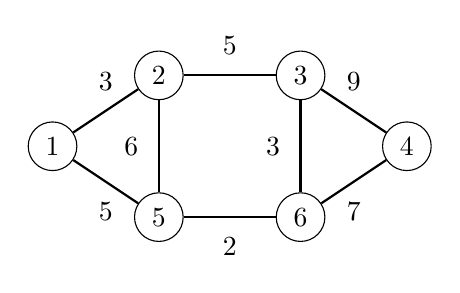
\begin{tikzpicture}[scale=0.9]
\node[draw, circle] (1) at (1.5,2) {$1$};
\node[draw, circle] (2) at (3,3) {$2$};
\node[draw, circle] (3) at (5,3) {$3$};
\node[draw, circle] (4) at (6.5,2) {$4$};
\node[draw, circle] (5) at (3,1) {$5$};
\node[draw, circle] (6) at (5,1) {$6$};
\path[draw,thick,-] (1) -- node[font=\small,label=above:3] {} (2);
\path[draw,thick,-] (2) -- node[font=\small,label=above:5] {} (3);
\path[draw,thick,-] (3) -- node[font=\small,label=above:9] {} (4);
\path[draw,thick,-] (1) -- node[font=\small,label=below:5] {} (5);
\path[draw,thick,-] (5) -- node[font=\small,label=below:2] {} (6);
\path[draw,thick,-] (6) -- node[font=\small,label=below:7] {} (4);
\path[draw,thick,-] (2) -- node[font=\small,label=left:6] {} (5);
\path[draw,thick,-] (3) -- node[font=\small,label=left:3] {} (6);
\end{tikzpicture}
\end{center}
例えば、1つの全域木は次のようになります。
\begin{center}
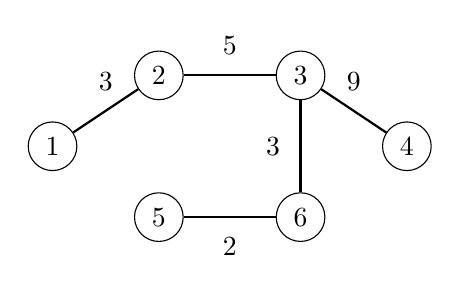
\begin{tikzpicture}[scale=0.9]
\node[draw, circle] (1) at (1.5,2) {$1$};
\node[draw, circle] (2) at (3,3) {$2$};
\node[draw, circle] (3) at (5,3) {$3$};
\node[draw, circle] (4) at (6.5,2) {$4$};
\node[draw, circle] (5) at (3,1) {$5$};
\node[draw, circle] (6) at (5,1) {$6$};
\path[draw,thick,-] (1) -- node[font=\small,label=above:3] {} (2);
\path[draw,thick,-] (2) -- node[font=\small,label=above:5] {} (3);
\path[draw,thick,-] (3) -- node[font=\small,label=above:9] {} (4);
\path[draw,thick,-] (5) -- node[font=\small,label=below:2] {} (6);
\path[draw,thick,-] (3) -- node[font=\small,label=left:3] {} (6);
\end{tikzpicture}
\end{center}

\index{minimum spanning tree}

全域木の重さとは、エッジの重みの合計です。
例えば、上記の全域木の重みは、$3+5+9+3+2 = 22$です。
\key{最小全域木(minimum spanning tree)}は、全ての全域木の中で最も重さが小さな全域木です。
先ほどの例では、次の最小全域木は重さが20です。

\begin{center}
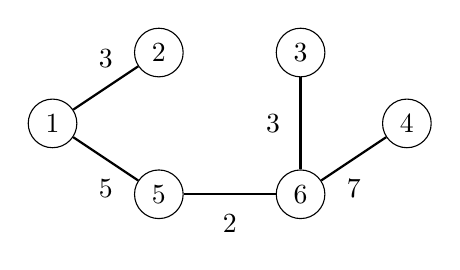
\begin{tikzpicture}[scale=0.9]
\node[draw, circle] (1) at (1.5,2) {$1$};
\node[draw, circle] (2) at (3,3) {$2$};
\node[draw, circle] (3) at (5,3) {$3$};
\node[draw, circle] (4) at (6.5,2) {$4$};
\node[draw, circle] (5) at (3,1) {$5$};
\node[draw, circle] (6) at (5,1) {$6$};

\path[draw,thick,-] (1) -- node[font=\small,label=above:3] {} (2);
\path[draw,thick,-] (1) -- node[font=\small,label=below:5] {} (5);
\path[draw,thick,-] (5) -- node[font=\small,label=below:2] {} (6);
\path[draw,thick,-] (6) -- node[font=\small,label=below:7] {} (4);
\path[draw,thick,-] (3) -- node[font=\small,label=left:3] {} (6);
\end{tikzpicture}
\end{center}

\index{maximum spanning tree}

\key{最大全域木(maximum spanning tree)}
は重さが最大となる木です。先の例では次のように重さ32の最大全域木ができます。

\begin{center}
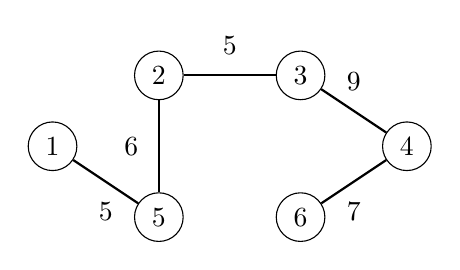
\begin{tikzpicture}[scale=0.9]
\node[draw, circle] (1) at (1.5,2) {$1$};
\node[draw, circle] (2) at (3,3) {$2$};
\node[draw, circle] (3) at (5,3) {$3$};
\node[draw, circle] (4) at (6.5,2) {$4$};
\node[draw, circle] (5) at (3,1) {$5$};
\node[draw, circle] (6) at (5,1) {$6$};
\path[draw,thick,-] (2) -- node[font=\small,label=above:5] {} (3);
\path[draw,thick,-] (3) -- node[font=\small,label=above:9] {} (4);
\path[draw,thick,-] (1) -- node[font=\small,label=below:5] {} (5);
\path[draw,thick,-] (6) -- node[font=\small,label=below:7] {} (4);
\path[draw,thick,-] (2) -- node[font=\small,label=left:6] {} (5);
\end{tikzpicture}
\end{center}

ここで、最小全域木・最大全域木になるグラフ(木)は複数存在することがあります。
これらの全域木は貪欲な方法で求めることができます。この章では、2つのアルゴリズムについて説明します。
説明上、最小全域木のみに絞って説明を行いますが、最大全域木の場合は処理する辺の順を逆とすれば良いです。

\section{クラスカル法 - Kruskal's algorithm}

\index{Kruskal's algorithm}

\key{Kruskalのアルゴリズム}
\footnote{このアルゴリズムは1956年にJ. B. Kruskalによって発表された \cite{kru56}.}
は次のように動作します。
まず、グラフのノードだけを持ち、エッジを含みません。次に、このアルゴリズムは、重みが小さい順にエッジを調べ、
サイクルを作らない場合は常にグラフにエッジを追加します。
このアルゴリズムは、木を連結成分を保持してながら行います。
初期状態は、各ノードは別々の連結成分に属している。
木にエッジを追加する時、その2つの成分を結合します。
最後にすべてのノードは同じ成分に属し、最小全域木となります。

\subsubsection{例}

\begin{samepage}
次のグラフを考えます。
\begin{center}
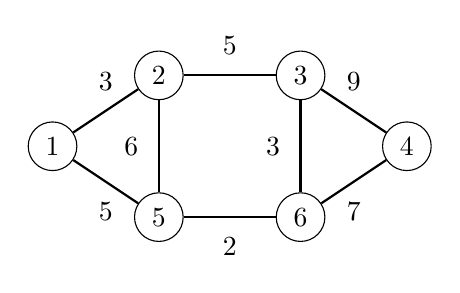
\begin{tikzpicture}[scale=0.9]
\node[draw, circle] (1) at (1.5,2) {$1$};
\node[draw, circle] (2) at (3,3) {$2$};
\node[draw, circle] (3) at (5,3) {$3$};
\node[draw, circle] (4) at (6.5,2) {$4$};
\node[draw, circle] (5) at (3,1) {$5$};
\node[draw, circle] (6) at (5,1) {$6$};
\path[draw,thick,-] (1) -- node[font=\small,label=above:3] {} (2);
\path[draw,thick,-] (2) -- node[font=\small,label=above:5] {} (3);
\path[draw,thick,-] (3) -- node[font=\small,label=above:9] {} (4);
\path[draw,thick,-] (1) -- node[font=\small,label=below:5] {} (5);
\path[draw,thick,-] (5) -- node[font=\small,label=below:2] {} (6);
\path[draw,thick,-] (6) -- node[font=\small,label=below:7] {} (4);
\path[draw,thick,-] (2) -- node[font=\small,label=left:6] {} (5);
\path[draw,thick,-] (3) -- node[font=\small,label=left:3] {} (6);
\end{tikzpicture}
\end{center}
\end{samepage}

\begin{samepage}
最初に全てのエッジを重みが小さい順にソートします。

\begin{tabular}{ll}
\\
edge & weight \\
\hline
5--6 & 2 \\
1--2 & 3 \\
3--6 & 3 \\
1--5 & 5 \\
2--3 & 5 \\
2--5 & 6 \\
4--6 & 7 \\
3--4 & 9 \\
\\
\end{tabular}
\end{samepage}

リストを上から処理し、各辺が2つの別の連結成分を結合するなら、その辺を接続します。

\begin{center}
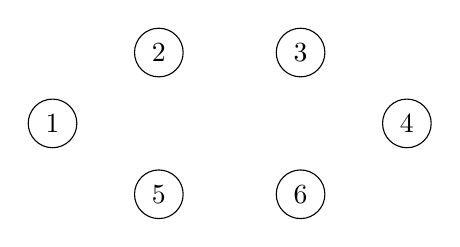
\begin{tikzpicture}[scale=0.9]
\node[draw, circle] (1) at (1.5,2) {$1$};
\node[draw, circle] (2) at (3,3) {$2$};
\node[draw, circle] (3) at (5,3) {$3$};
\node[draw, circle] (4) at (6.5,2) {$4$};
\node[draw, circle] (5) at (3,1) {$5$};
\node[draw, circle] (6) at (5,1) {$6$};
%\path[draw,thick,-] (1) -- node[font=\small,label=above:3] {} (2);
%\path[draw,thick,-] (2) -- node[font=\small,label=above:5] {} (3);
%\path[draw,thick,-] (3) -- node[font=\small,label=above:9] {} (4);
%\path[draw,thick,-] (1) -- node[font=\small,label=below:5] {} (5);
%\path[draw,thick,-] (5) -- node[font=\small,label=below:2] {} (6);
%\path[draw,thick,-] (6) -- node[font=\small,label=below:7] {} (4);
%\path[draw,thick,-] (2) -- node[font=\small,label=left:6] {} (5);
%\path[draw,thick,-] (3) -- node[font=\small,label=left:3] {} (6);
\end{tikzpicture}
\end{center}
まず、5--6 の処理は$\{5\}$ と $\{6\}$を連結し、
$\{5,6\}$とします。

\begin{center}
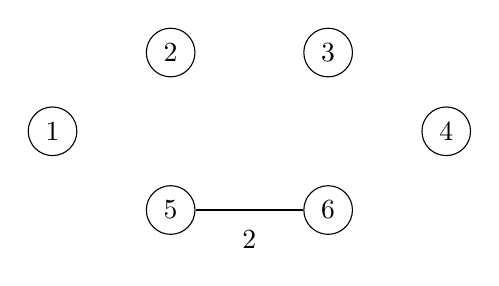
\begin{tikzpicture}
\node[draw, circle] (1) at (1.5,2) {$1$};
\node[draw, circle] (2) at (3,3) {$2$};
\node[draw, circle] (3) at (5,3) {$3$};
\node[draw, circle] (4) at (6.5,2) {$4$};
\node[draw, circle] (5) at (3,1) {$5$};
\node[draw, circle] (6) at (5,1) {$6$};

%\path[draw,thick,-] (1) -- node[font=\small,label=above:3] {} (2);
%\path[draw,thick,-] (2) -- node[font=\small,label=above:5] {} (3);
%\path[draw,thick,-] (3) -- node[font=\small,label=above:9] {} (4);
%\path[draw,thick,-] (1) -- node[font=\small,label=below:5] {} (5);
\path[draw,thick,-] (5) -- node[font=\small,label=below:2] {} (6);
%\path[draw,thick,-] (6) -- node[font=\small,label=below:7] {} (4);
%\path[draw,thick,-] (2) -- node[font=\small,label=left:6] {} (5);
%\path[draw,thick,-] (3) -- node[font=\small,label=left:3] {} (6);
\end{tikzpicture}
\end{center}
同じように、 1--2, 3--6, 1--5 が接続されます。

\begin{center}
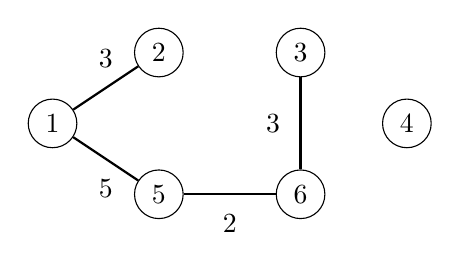
\begin{tikzpicture}[scale=0.9]
\node[draw, circle] (1) at (1.5,2) {$1$};
\node[draw, circle] (2) at (3,3) {$2$};
\node[draw, circle] (3) at (5,3) {$3$};
\node[draw, circle] (4) at (6.5,2) {$4$};
\node[draw, circle] (5) at (3,1) {$5$};
\node[draw, circle] (6) at (5,1) {$6$};

\path[draw,thick,-] (1) -- node[font=\small,label=above:3] {} (2);
%\path[draw,thick,-] (2) -- node[font=\small,label=above:5] {} (3);
%\path[draw,thick,-] (3) -- node[font=\small,label=above:9] {} (4);
\path[draw,thick,-] (1) -- node[font=\small,label=below:5] {} (5);
\path[draw,thick,-] (5) -- node[font=\small,label=below:2] {} (6);
%\path[draw,thick,-] (6) -- node[font=\small,label=below:7] {} (4);
%\path[draw,thick,-] (2) -- node[font=\small,label=left:6] {} (5);
\path[draw,thick,-] (3) -- node[font=\small,label=left:3] {} (6);
\end{tikzpicture}
\end{center}

これらのステップの後、ほとんどの連結成分は結合され、2つの連結成分が存在します。
$\{1,2,3,5,6\}$と$\{4\}$です。

次に処理するのは2--3ですが、同じ連結成分に含まれるので接続しません。 2--5も同様です。

\begin{samepage}
最後に、4--6が接続されます。

\begin{center}
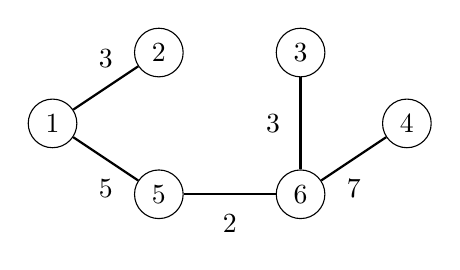
\begin{tikzpicture}[scale=0.9]
\node[draw, circle] (1) at (1.5,2) {$1$};
\node[draw, circle] (2) at (3,3) {$2$};
\node[draw, circle] (3) at (5,3) {$3$};
\node[draw, circle] (4) at (6.5,2) {$4$};
\node[draw, circle] (5) at (3,1) {$5$};
\node[draw, circle] (6) at (5,1) {$6$};

\path[draw,thick,-] (1) -- node[font=\small,label=above:3] {} (2);
%\path[draw,thick,-] (2) -- node[font=\small,label=above:5] {} (3);
%\path[draw,thick,-] (3) -- node[font=\small,label=above:9] {} (4);
\path[draw,thick,-] (1) -- node[font=\small,label=below:5] {} (5);
\path[draw,thick,-] (5) -- node[font=\small,label=below:2] {} (6);
\path[draw,thick,-] (6) -- node[font=\small,label=below:7] {} (4);
%\path[draw,thick,-] (2) -- node[font=\small,label=left:6] {} (5);
\path[draw,thick,-] (3) -- node[font=\small,label=left:3] {} (6);
\end{tikzpicture}
\end{center}
\end{samepage}

これで全ての点が同じ連結成分に含まれるので処理を終えます。
これにより、重さが$2+3+3+5+7=20$の最小全域木ができました。

\subsubsection{なぜこれで良いか?}

なぜこのアルゴリズムが有効なのか?つまり、これでなぜ最小全域木が求められるのでしょう?
最小の重みの辺が含まれないことを考えます。
例えば、先ほどの例で最小重みの辺5--6 が含まれないとします。
そのようなグラフは複数考えられますが、例えば次のような木を考えましょう。

\begin{center}
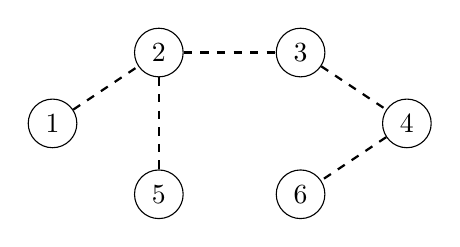
\begin{tikzpicture}[scale=0.9]
\node[draw, circle] (1) at (1.5,2) {$1$};
\node[draw, circle] (2) at (3,3) {$2$};
\node[draw, circle] (3) at (5,3) {$3$};
\node[draw, circle] (4) at (6.5,2) {$4$};
\node[draw, circle] (5) at (3,1) {$5$};
\node[draw, circle] (6) at (5,1) {$6$};

\path[draw,thick,-,dashed] (1) -- (2);
\path[draw,thick,-,dashed] (2) -- (5);
\path[draw,thick,-,dashed] (2) -- (3);
\path[draw,thick,-,dashed] (3) -- (4);
\path[draw,thick,-,dashed] (4) -- (6);
\end{tikzpicture}
\end{center}


しかし、この木が最小全域木ではありません。
木からある辺を取り除き、5--6に置き換えることができ、さらに重さの小さな木ができます。

\begin{center}
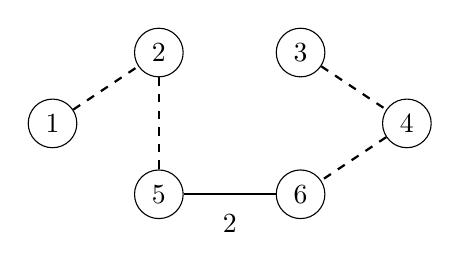
\begin{tikzpicture}[scale=0.9]
\node[draw, circle] (1) at (1.5,2) {$1$};
\node[draw, circle] (2) at (3,3) {$2$};
\node[draw, circle] (3) at (5,3) {$3$};
\node[draw, circle] (4) at (6.5,2) {$4$};
\node[draw, circle] (5) at (3,1) {$5$};
\node[draw, circle] (6) at (5,1) {$6$};

\path[draw,thick,-,dashed] (1) -- (2);
\path[draw,thick,-,dashed] (2) -- (5);
\path[draw,thick,-,dashed] (3) -- (4);
\path[draw,thick,-,dashed] (4) -- (6);
\path[draw,thick,-] (5) -- node[font=\small,label=below:2] {} (6);
\end{tikzpicture}
\end{center}

For this reason, it is always optimal
to include the minimum weight edge
in the tree to produce a minimum spanning tree.
Using a similar argument, we can show that it
is also optimal to add the next edge in weight order
to the tree, and so on.
Hence, Kruskal's algorithm works correctly and
always produces a minimum spanning tree.

\subsubsection{Implementation}

When implementing Kruskal's algorithm,
it is convenient to use
the edge list representation of the graph.
The first phase of the algorithm sorts the
edges in the list in $O(m \log m)$ time.
After this, the second phase of the algorithm
builds the minimum spanning tree as follows:

\begin{lstlisting}
for (...) {
  if (!same(a,b)) unite(a,b);
}
\end{lstlisting}

The loop goes through the edges in the list
and always processes an edge $a$--$b$
where $a$ and $b$ are two nodes.
Two functions are needed:
the function \texttt{same} determines
if $a$ and $b$ are in the same component,
and the function \texttt{unite}
joins the components that contain $a$ and $b$.

The problem is how to efficiently implement
the functions \texttt{same} and \texttt{unite}.
One possibility is to implement the function
\texttt{same} as a graph traversal and check if
we can get from node $a$ to node $b$.
However, the time complexity of such a function
would be $O(n+m)$
and the resulting algorithm would be slow,
because the function \texttt{same} will be called for each edge in the graph.

We will solve the problem using a union-find structure
that implements both functions in $O(\log n)$ time.
Thus, the time complexity of Kruskal's algorithm
will be $O(m \log n)$ after sorting the edge list.

\section{Union-find structure}

\index{union-find structure}

A \key{union-find structure} maintains
a collection of sets.
The sets are disjoint, so no element
belongs to more than one set.
Two $O(\log n)$ time operations are supported:
the \texttt{unite} operation joins two sets,
and the \texttt{find} operation finds the representative
of the set that contains a given element\footnote{The structure presented here
was introduced in 1971 by J. D. Hopcroft and J. D. Ullman \cite{hop71}.
Later, in 1975, R. E. Tarjan studied a more sophisticated variant
of the structure \cite{tar75} that is discussed in many algorithm
textbooks nowadays.}.

\subsubsection{Structure}

In a union-find structure, one element in each set
is the representative of the set,
and there is a chain from any other element of the
set to the representative.
For example, assume that the sets are
$\{1,4,7\}$, $\{5\}$ and $\{2,3,6,8\}$:
\begin{center}
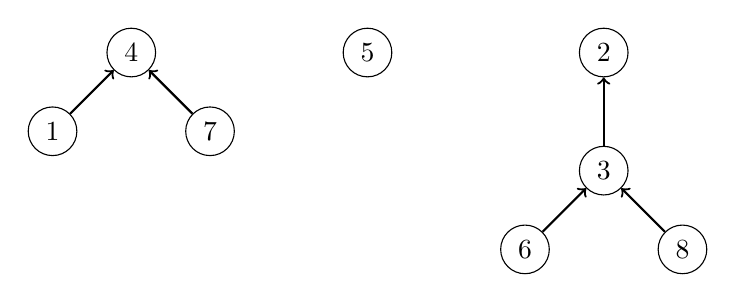
\begin{tikzpicture}
\node[draw, circle] (1) at (0,-1) {$1$};
\node[draw, circle] (2) at (7,0) {$2$};
\node[draw, circle] (3) at (7,-1.5) {$3$};
\node[draw, circle] (4) at (1,0) {$4$};
\node[draw, circle] (5) at (4,0) {$5$};
\node[draw, circle] (6) at (6,-2.5) {$6$};
\node[draw, circle] (7) at (2,-1) {$7$};
\node[draw, circle] (8) at (8,-2.5) {$8$};

\path[draw,thick,->] (1) -- (4);
\path[draw,thick,->] (7) -- (4);

\path[draw,thick,->] (3) -- (2);
\path[draw,thick,->] (6) -- (3);
\path[draw,thick,->] (8) -- (3);

\end{tikzpicture}
\end{center}
In this case the representatives
of the sets are 4, 5 and 2.
We can find the representative of any element
by following the chain that begins at the element.
For example, the element 2 is the representative
for the element 6, because
we follow the chain $6 \rightarrow 3 \rightarrow 2$.
Two elements belong to the same set exactly when
their representatives are the same.

Two sets can be joined by connecting the
representative of one set to the
representative of the other set.
For example, the sets
$\{1,4,7\}$ and $\{2,3,6,8\}$
can be joined as follows:
\begin{center}
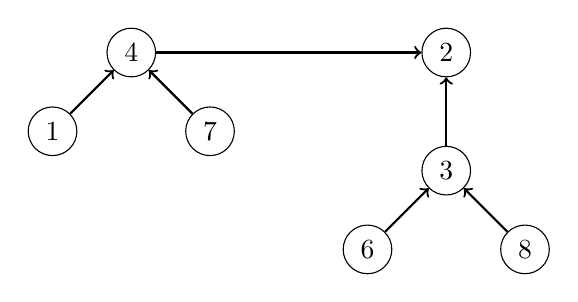
\begin{tikzpicture}
\node[draw, circle] (1) at (2,-1) {$1$};
\node[draw, circle] (2) at (7,0) {$2$};
\node[draw, circle] (3) at (7,-1.5) {$3$};
\node[draw, circle] (4) at (3,0) {$4$};
\node[draw, circle] (6) at (6,-2.5) {$6$};
\node[draw, circle] (7) at (4,-1) {$7$};
\node[draw, circle] (8) at (8,-2.5) {$8$};

\path[draw,thick,->] (1) -- (4);
\path[draw,thick,->] (7) -- (4);

\path[draw,thick,->] (3) -- (2);
\path[draw,thick,->] (6) -- (3);
\path[draw,thick,->] (8) -- (3);

\path[draw,thick,->] (4) -- (2);
\end{tikzpicture}
\end{center}

The resulting set contains the elements
$\{1,2,3,4,6,7,8\}$.
From this on, the element 2 is the representative
for the entire set and the old representative 4
points to the element 2.

The efficiency of the union-find structure depends on
how the sets are joined.
It turns out that we can follow a simple strategy:
always connect the representative of the
\emph{smaller} set to the representative of the \emph{larger} set
(or if the sets are of equal size,
we can make an arbitrary choice).
Using this strategy, the length of any chain
will be $O(\log n)$, so we can
find the representative of any element
efficiently by following the corresponding chain.

\subsubsection{Implementation}

The union-find structure can be implemented
using arrays.
In the following implementation,
the array \texttt{link} contains for each element
the next element
in the chain or the element itself if it is
a representative,
and the array \texttt{size} indicates for each representative
the size of the corresponding set.

Initially, each element belongs to a separate set:
\begin{lstlisting}
for (int i = 1; i <= n; i++) link[i] = i;
for (int i = 1; i <= n; i++) size[i] = 1;
\end{lstlisting}

The function \texttt{find} returns
the representative for an element $x$.
The representative can be found by following
the chain that begins at $x$.

\begin{lstlisting}
int find(int x) {
    while (x != link[x]) x = link[x];
    return x;
}
\end{lstlisting}

The function \texttt{same} checks
whether elements $a$ and $b$ belong to the same set.
This can easily be done by using the
function \texttt{find}:

\begin{lstlisting}
bool same(int a, int b) {
    return find(a) == find(b);
}
\end{lstlisting}

\begin{samepage}
The function \texttt{unite} joins the sets
that contain elements $a$ and $b$
(the elements have to be in different sets).
The function first finds the representatives
of the sets and then connects the smaller
set to the larger set.

\begin{lstlisting}
void unite(int a, int b) {
    a = find(a);
    b = find(b);
    if (size[a] < size[b]) swap(a,b);
    size[a] += size[b];
    link[b] = a;
}
\end{lstlisting}
\end{samepage}

The time complexity of the function \texttt{find}
is $O(\log n)$ assuming that the length of each
chain is $O(\log n)$.
In this case, the functions \texttt{same} and \texttt{unite}
also work in $O(\log n)$ time.
The function \texttt{unite} makes sure that the
length of each chain is $O(\log n)$ by connecting
the smaller set to the larger set.

\section{Prim's algorithm}

\index{Prim's algorithm}

\key{Prim's algorithm}\footnote{The algorithm is
named after R. C. Prim who published it in 1957 \cite{pri57}.
However, the same algorithm was discovered already in 1930
by V. Jarník.} is an alternative method
for finding a minimum spanning tree.
The algorithm first adds an arbitrary node
to the tree.
After this, the algorithm always chooses
a minimum-weight edge that
adds a new node to the tree.
Finally, all nodes have been added to the tree
and a minimum spanning tree has been found.

Prim's algorithm resembles Dijkstra's algorithm.
The difference is that Dijkstra's algorithm always
selects an edge whose distance from the starting
node is minimum, but Prim's algorithm simply selects
the minimum weight edge that adds a new node to the tree.

\subsubsection{Example}

Let us consider how Prim's algorithm works
in the following graph:

\begin{center}
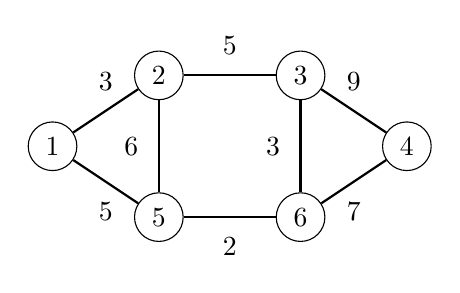
\begin{tikzpicture}[scale=0.9]
\node[draw, circle] (1) at (1.5,2) {$1$};
\node[draw, circle] (2) at (3,3) {$2$};
\node[draw, circle] (3) at (5,3) {$3$};
\node[draw, circle] (4) at (6.5,2) {$4$};
\node[draw, circle] (5) at (3,1) {$5$};
\node[draw, circle] (6) at (5,1) {$6$};
\path[draw,thick,-] (1) -- node[font=\small,label=above:3] {} (2);
\path[draw,thick,-] (2) -- node[font=\small,label=above:5] {} (3);
\path[draw,thick,-] (3) -- node[font=\small,label=above:9] {} (4);
\path[draw,thick,-] (1) -- node[font=\small,label=below:5] {} (5);
\path[draw,thick,-] (5) -- node[font=\small,label=below:2] {} (6);
\path[draw,thick,-] (6) -- node[font=\small,label=below:7] {} (4);
\path[draw,thick,-] (2) -- node[font=\small,label=left:6] {} (5);
\path[draw,thick,-] (3) -- node[font=\small,label=left:3] {} (6);

%\path[draw=red,thick,-,line width=2pt] (5) -- (6);
\end{tikzpicture}
\end{center}
Initially, there are no edges between the nodes:
\begin{center}
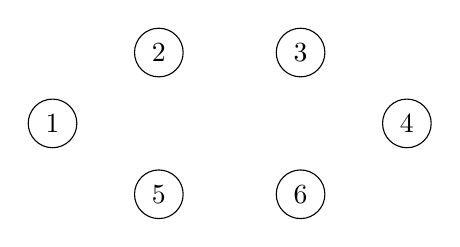
\begin{tikzpicture}[scale=0.9]
\node[draw, circle] (1) at (1.5,2) {$1$};
\node[draw, circle] (2) at (3,3) {$2$};
\node[draw, circle] (3) at (5,3) {$3$};
\node[draw, circle] (4) at (6.5,2) {$4$};
\node[draw, circle] (5) at (3,1) {$5$};
\node[draw, circle] (6) at (5,1) {$6$};
%\path[draw,thick,-] (1) -- node[font=\small,label=above:3] {} (2);
%\path[draw,thick,-] (2) -- node[font=\small,label=above:5] {} (3);
%\path[draw,thick,-] (3) -- node[font=\small,label=above:9] {} (4);
%\path[draw,thick,-] (1) -- node[font=\small,label=below:5] {} (5);
%\path[draw,thick,-] (5) -- node[font=\small,label=below:2] {} (6);
%\path[draw,thick,-] (6) -- node[font=\small,label=below:7] {} (4);
%\path[draw,thick,-] (2) -- node[font=\small,label=left:6] {} (5);
%\path[draw,thick,-] (3) -- node[font=\small,label=left:3] {} (6);
\end{tikzpicture}
\end{center}
An arbitrary node can be the starting node,
so let us choose node 1.
First, we add node 2 that is connected by
an edge of weight 3:
\begin{center}
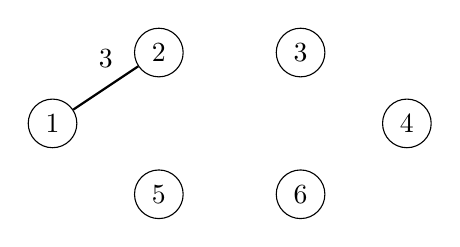
\begin{tikzpicture}[scale=0.9]
\node[draw, circle] (1) at (1.5,2) {$1$};
\node[draw, circle] (2) at (3,3) {$2$};
\node[draw, circle] (3) at (5,3) {$3$};
\node[draw, circle] (4) at (6.5,2) {$4$};
\node[draw, circle] (5) at (3,1) {$5$};
\node[draw, circle] (6) at (5,1) {$6$};
\path[draw,thick,-] (1) -- node[font=\small,label=above:3] {} (2);
%\path[draw,thick,-] (2) -- node[font=\small,label=above:5] {} (3);
%\path[draw,thick,-] (3) -- node[font=\small,label=above:9] {} (4);
%\path[draw,thick,-] (1) -- node[font=\small,label=below:5] {} (5);
%\path[draw,thick,-] (5) -- node[font=\small,label=below:2] {} (6);
%\path[draw,thick,-] (6) -- node[font=\small,label=below:7] {} (4);
%\path[draw,thick,-] (2) -- node[font=\small,label=left:6] {} (5);
%\path[draw,thick,-] (3) -- node[font=\small,label=left:3] {} (6);
\end{tikzpicture}
\end{center}

After this, there are two edges with weight 5,
so we can add either node 3 or node 5 to the tree.
Let us add node 3 first:
\begin{center}
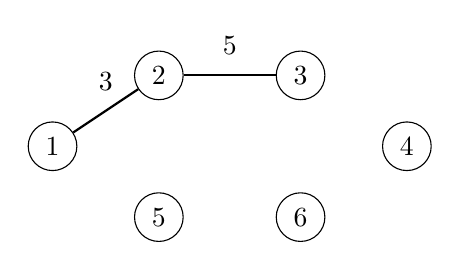
\begin{tikzpicture}[scale=0.9]
\node[draw, circle] (1) at (1.5,2) {$1$};
\node[draw, circle] (2) at (3,3) {$2$};
\node[draw, circle] (3) at (5,3) {$3$};
\node[draw, circle] (4) at (6.5,2) {$4$};
\node[draw, circle] (5) at (3,1) {$5$};
\node[draw, circle] (6) at (5,1) {$6$};
\path[draw,thick,-] (1) -- node[font=\small,label=above:3] {} (2);
\path[draw,thick,-] (2) -- node[font=\small,label=above:5] {} (3);
%\path[draw,thick,-] (3) -- node[font=\small,label=above:9] {} (4);
%\path[draw,thick,-] (1) -- node[font=\small,label=below:5] {} (5);
%\path[draw,thick,-] (5) -- node[font=\small,label=below:2] {} (6);
%\path[draw,thick,-] (6) -- node[font=\small,label=below:7] {} (4);
%\path[draw,thick,-] (2) -- node[font=\small,label=left:6] {} (5);
%\path[draw,thick,-] (3) -- node[font=\small,label=left:3] {} (6);
\end{tikzpicture}
\end{center}

\begin{samepage}
The process continues until all nodes have been included in the tree:
\begin{center}
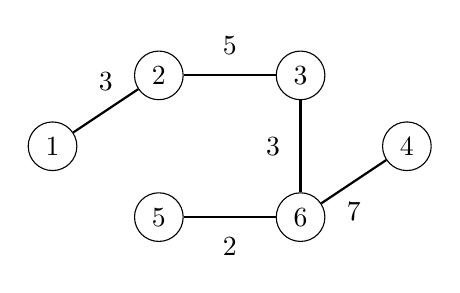
\begin{tikzpicture}[scale=0.9]
\node[draw, circle] (1) at (1.5,2) {$1$};
\node[draw, circle] (2) at (3,3) {$2$};
\node[draw, circle] (3) at (5,3) {$3$};
\node[draw, circle] (4) at (6.5,2) {$4$};
\node[draw, circle] (5) at (3,1) {$5$};
\node[draw, circle] (6) at (5,1) {$6$};
\path[draw,thick,-] (1) -- node[font=\small,label=above:3] {} (2);
\path[draw,thick,-] (2) -- node[font=\small,label=above:5] {} (3);
%\path[draw,thick,-] (3) -- node[font=\small,label=above:9] {} (4);
%\path[draw,thick,-] (1) -- node[font=\small,label=below:5] {} (5);
\path[draw,thick,-] (5) -- node[font=\small,label=below:2] {} (6);
\path[draw,thick,-] (6) -- node[font=\small,label=below:7] {} (4);
%\path[draw,thick,-] (2) -- node[font=\small,label=left:6] {} (5);
\path[draw,thick,-] (3) -- node[font=\small,label=left:3] {} (6);
\end{tikzpicture}
\end{center}
\end{samepage}

\subsubsection{Implementation}

Like Dijkstra's algorithm, Prim's algorithm can be
efficiently implemented using a priority queue.
The priority queue should contain all nodes
that can be connected to the current component using
a single edge, in increasing order of the weights
of the corresponding edges.

The time complexity of Prim's algorithm is
$O(n + m \log m)$ that equals the time complexity
of Dijkstra's algorithm.
In practice, Prim's and Kruskal's algorithms
are both efficient, and the choice of the algorithm
is a matter of taste.
Still, most competitive programmers use Kruskal's algorithm.
